\documentclass[12pt,twoside]{article}
\usepackage[a4paper,width=150mm,top=25mm,bottom=25mm, bindingoffset=6mm]{geometry}
%\usepackage{fancyhdr}
%\pagestyle{fancy}

\usepackage[]{biblatex}
\addbibresource{sources.bib}

\usepackage{caption}
\usepackage{subcaption}

\usepackage{listings}
\usepackage{graphicx} 
\usepackage[ngerman]{babel}
\usepackage[utf8]{inputenc}
\usepackage[T1]{fontenc}    
\usepackage{amsmath}
\usepackage{float}
\usepackage{url}

\lstset{language=Python}
\newlength{\swidth}
\setlength{\swidth}{0.6\textwidth}

\pagestyle{plain}

\title{deepLID}
\author{Joel André}
\date{\today{}}

\begin{document}
	
	\begin{titlepage}
    \begin{center}
        \vspace*{1cm}
        
        \Huge
        \textbf{Identifikation gesprochener Sprache mit Deep Learning}
            
        \vspace{4cm}
        
        
\includegraphics[width=0.4\textwidth]{assets/front.png}
        
         \vspace{4cm}
        
        \textbf{Joel André}
        \vspace{2.5cm}
        
        
        \Large
        Maturaarbeit\\
        Betreut von
        Beni Keller
        
        \vspace{0.8cm}
        
        
        Kantonsschule Zug\\
        2019
        
    \end{center}
\end{titlepage}
	
	\tableofcontents
	\newpage
	
	\section{Einleitung}
	\section{Deep learning}
Die Begriffe \textit{Deep Learning}, \textit{maschinelles Lernen} und \textit{künstliche Intelligenz} werden oft fälschlicherweise auswechselbar verwendet. Es gibt allerdings eine ganz klare, und für das Verständnis wichtige Hierarchie zwischen den Wörtern. Um Klarheit zu verschaffen werden darum alle Gebiete aufgeführt.

\begin{figure}[hbt]
	\centering
		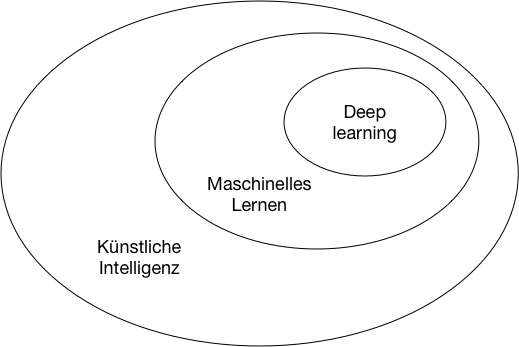
\includegraphics[width=0.6\textwidth]{assets/hierarchy.png}
	\caption{Künstliche Intelligenz, Maschinelles Lernen und Deep Learning}
	\label{img:hierarchy}
\end{figure}

Das Gebiet der künstlichen Intelligenz gibt es schon so lange wie den Computer selbst. Die Frage, wie schlau ein Computer werden kann, beschäftigt uns bis heute. Als anerkannte Definition für KI gilt, das Bestreben intellektuelle Aufgaben, die normalerweise von Menschen gelöst werden, zu automatisieren.\index{Künstliche Intelligenz (KI)}

Erste Erfolge erreichte man zum Beispiel mit Schachcomputern, die handgeschriebene Regeln befolgten. Diese Form von künstlicher Intelligenz hat aber schnell Grenzen, da viele Prozesse schlicht zu komplex sind, um sie unter angemessenem Aufwand mit Regeln zu beschreiben. Um dieses Problem zu lösen, erfand man maschinelles Lernens. \index{Maschinelles Lernen}

Der Ablauf von maschinellem Lernen ist grundlegend anders als konventionelles Programmieren. Der Entwickler muss  keinen Programmcode mit festen Regeln schreiben, im Gegenteil: Er liefert dem Computer Eingabe und Ausgabe, und der Computer lernt die Regeln selbst. Kurzgesagt lernt das System aus Beispielen Muster zu erkennen. Maschinelles Lernen blühte erst in den 90'er Jahren auf, wurde aber schnell zum grössten Teilgebiet der künstlichen Intelligenz.

Beim maschinellem Lernen, lernt die Software im Grunde eine nützlichere Darstellungsweise der Daten bzw. der Eingabe. Anhand dieser anderen Darstellungsweise kann der Computer die Antwort einfach erkennen. Wenn der Computer stufenweise nützlichere Repräsentationen bestimmt, kann er zunehmend komplexe Probleme, in einfacheren Zwischenschritten lösen. Genau das ist \textit{Deep Learning}. Das \textit{Deep} entspringt der grossen Anzahl an aufeinanderfolgenden Repräsentation. Deep Learning bezeichnet das Konzept von stufenweisem Lernen und nicht eine Methode selbst. Eine weit verbreitete Methode sind allerdings \textit{tiefe künstliche neuronale Netze}.\parencite[vgl.][]{chollet} \index{Deep Learning}

\subsection{Künstliche neuronale Netze}

\textit{Künstliche neuronale Netze} \index{Künstliche neuronale Netze}hat man sich, wie der Name schon preisgibt, von der Natur abgesehen. Ähnlich wie in unserem Gehirn gibt es Neuronen bzw. Knoten und dazwischenliegende Verbindungen. Die \say{Intelligenz} entsteht erst aus dem Zusammenspiel tausender Neuronen. Künstliche Neurone Netze haben sich mittlerweile so stark weiterentwickelt, dass sie nebst der ursprünglichen Idee, nichts mehr mit der biologischen Variante gemeinsam haben. \\

Der Wert eines Knotens/Neurons ist abhängig von der Summe aller seiner eingehenden Verbindungen. Die Abhängigkeit wird duch die Aktivierungsfunktion $\sigma$ definiert. Die Aktivierungssfunktion ist wichtig, damit das Netzwerk jede mögliche Funktion abbilden kann. Es ist bewiesen dass neuronalen Netze universelle Approximatoren sind\parencite[][Kap. 4]{universal}. Eine bekannte Aktivierungsfunktion ist zum Beispiel die \textit{ReLU} \index{ReLU}Funktion. Die ReLU Funktion unterdrückt negative Werte, bzw. sie ist null für Werte kleiner als null.   \parencite{neuronale_netze} 
$$\sigma(x) = \text{ReLU}(x) = \text{max}(0, x)$$

Der Wert einer eingehenden Verbindung ist proportional zum Wert des Herkunfsknoten, bzw. des Knoten woher die Verbindung kommt. Der Wert des Herkunfsknoten wird multipliziert mit dem Gewicht der Verbindung: $w$. Die Gewichte der Verbindungen sind die Parameter des Netzwerks. Intuitiv kann man sich vorstellen, dass das Netzwerk lernt, wichtigeren Verbindungen grössere Gewichte zuzuordnen und Unwichtigen umgekehrt. Wenn man alles zusammensetzt ergibt sich für den Wert irgendeinen Knotens $o_i$ mit Vorgänger-Knoten $\boldsymbol{h}$ diese Formel:
$$ o_i = \sigma\Big(\sum_i h_i \cdot w_{i}\Big)$$
Mit dieser Formel propagieren sich die Werte der Anfangsknoten durch das ganze Netzwerk. Um das Prinzip anschaulicher zu machen, wird ein Beispiel-Durchlauf vorgeführt. Die verwendeten Gewichte und Eingaben sind willkürlich.

Die Aufgabe des vorgestellten Netzwerks ist es zum Beispiel, zwischen Hund und Katze zu unterscheiden. Die Eingaben $x_1$ und $x_2$ sind gewisse Merkmale des zu erkennenden Tieres. $1$ bedeutet, dass Tier besitzt das Attribut und $0$ das Gegenteil. Die Ausgabe $o$ beschreibt die Wahrscheinlichkeit, dass das Tier eine Katze ist. Daraus folgt, dass Werte $o>0.5$ für Katze stehen und Werte $o<0.5$ für Hunde.
\begin{figure}[hbt]
	\centering
		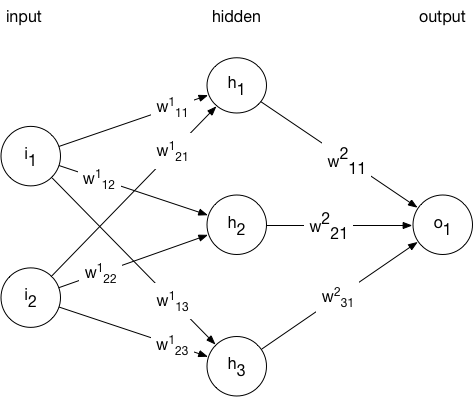
\includegraphics[width=0.85\textwidth]{assets/neural_net.png}
	\caption{Grafische Darstellung eines künstlichen neuronalen Netzwerks anhand eines Beispiels: Rote Zahlen sind festgesetzt und grüne Zahlen werden berechnet.}
	\label{img:neuralnet}
\end{figure}

Was bis jetzt berechnet wurde nennt man den \textit{Vorwärtspass}. Aus einer Eingabe wurde die Ausgabe berechnet. Daran war aber noch nichts intelligent. Erst jetzt können die Parameter der Funktion, die Gewichte, aus diesem Beispiel lernen (Siehe Abbildung \ref{img:anatomy}). Um diese zu verbessern braucht es eine \textit{Verlust Funktion} \index{Verlust Funktion}die uns angibt, wie weit die Ausgabe vom korrekten Ziel entfernt ist. Eine mögliche Verlust Funktion ist die absolute Differenz zwischen dem Ziel und der Ausgabe. Wenn man in oberen Beispiel davon ausgeht, dass die Eingabe wirklich zu einer Katze gehört, ergäbe sich:
$$ \text{Verlust}(output, target) = |target-output| = |1.0-0.747| = 0.253$$
Um den Verlustwert zu minimieren, passt das Netzwerk die Gewichte schrittweise an. Diesen Teil übernimmt der  \textit{Optimierer}. Ein einfacher Optimierer ist zum Beispiel das Gradientenverfahren. Details dazu befinden sich in \parencite{gradient}.

\begin{figure}[hbt]
	\centering
		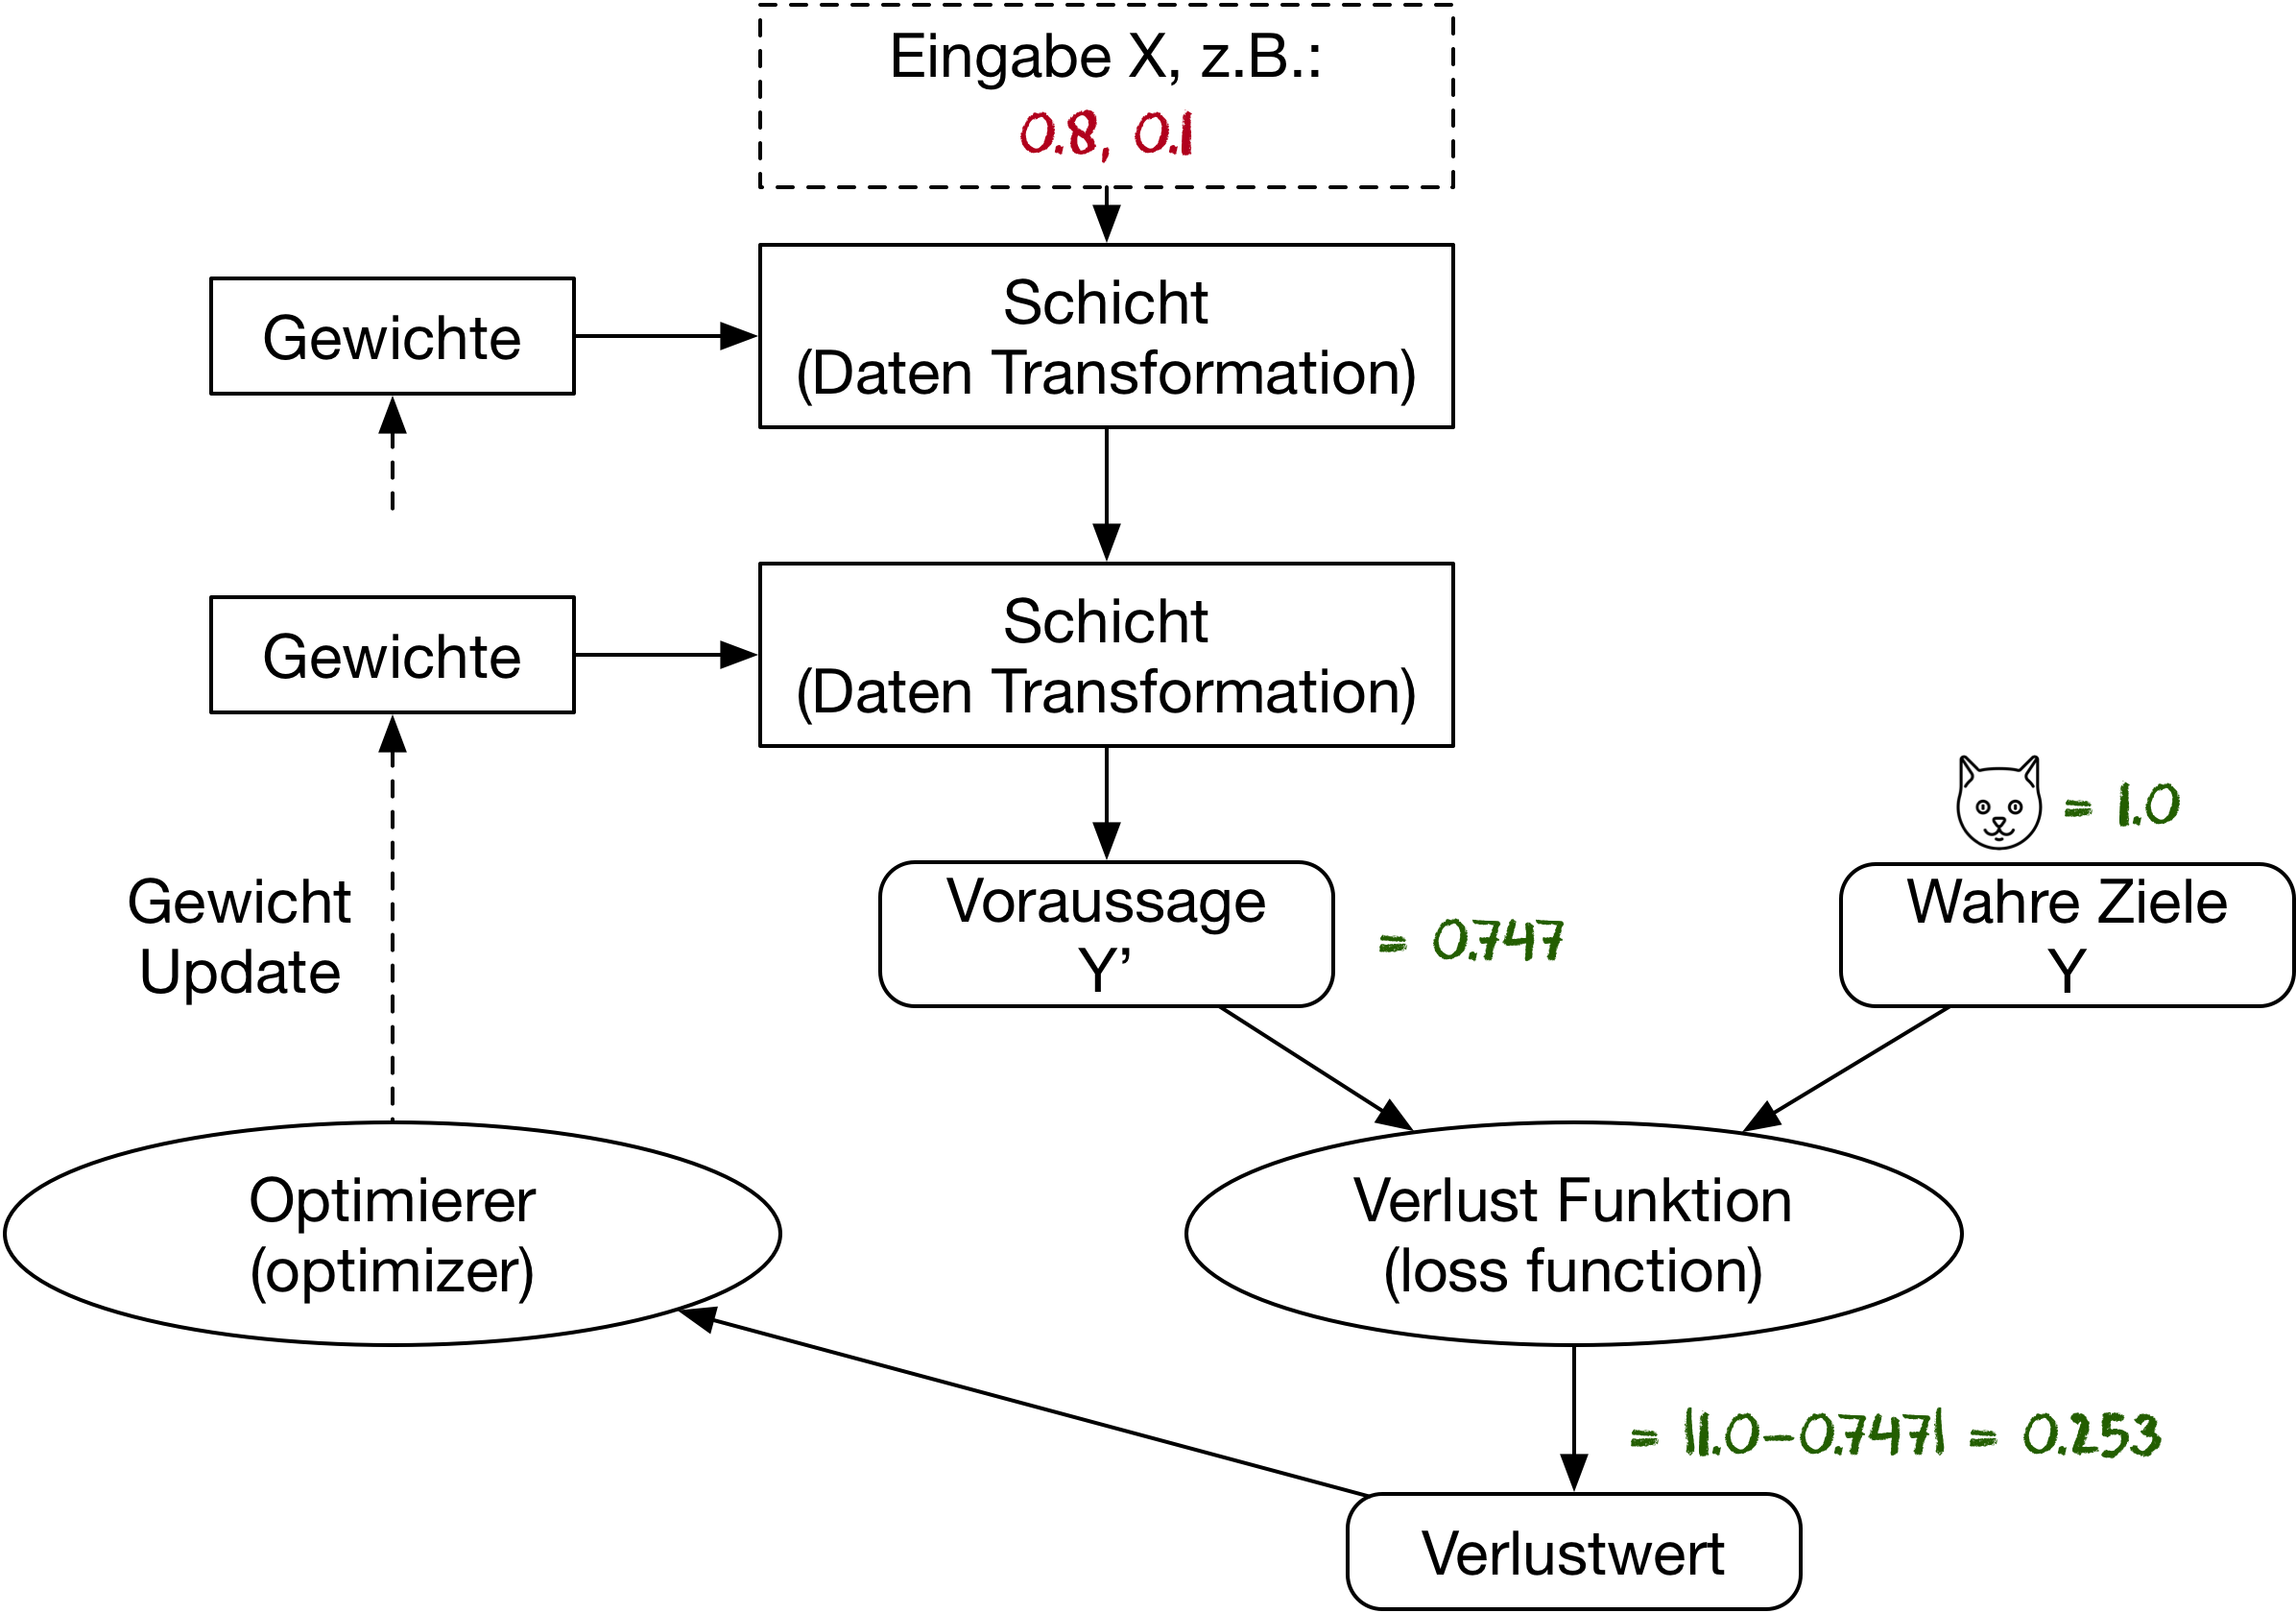
\includegraphics[width=0.8\textwidth]{assets/anatomy.png}
	\caption{Visuelle Darstellung des Lern-Prozesses anhand eines Beispiels}
	\label{img:anatomy}
\end{figure}

Da bei diesem Typ von neuronalen Netzwerken alle Knoten miteinander verbunden sind, wird es oft \textit{Dense Neural Network} \index{Dense Neural Network}genannt.
\\
Die mathematischen Operationen in einem neuronalen Netzwerk lassen sich alle als Matrizen-Operationen berechnen. Mit Matrizen kann der Computer auf einer Grafikkarte und mit einem BLAS \index{BLAS}(\textit{Basic linear algebra system}) sehr effizient rechnen \parencite{neuronale_netze} .


\subsection{Convolutional Neural Networks}
\textit{Convolutional Neural Networks} \index{Convolutional Neural Networks (CNN)}sind eine sehr weit verbreitete Methode im Feld von \textit{Computer Vision}. Der fundamentale Unterschied zwischen dem oben besprochenen \textit{dense network} und einem \textit{CNN} ist, dass ein \textit{CNN} lokale Muster erkennen kann, wo hingegen das vorherige Netzwerk nur globale Muster erkennen konnte. Das bedeutet, dass ein Muster, das an einer bestimmten Stelle angetroffen wird, an jeder anderen Stelle ebenfalls erkannt wird. \parencite{chollet}

Um das zu erlauben, teilen gewisse Verbindungen das gleiche Gewicht. In Abbildung \ref{img:conv} (Oberer Teil) sind das die gleichfarbigen Verbindungen. Weniger Gewichte führen zusätzlich dazu, dass das Netzwerk schneller lernen kann.
\begin{figure}[hbt]
	\centering
		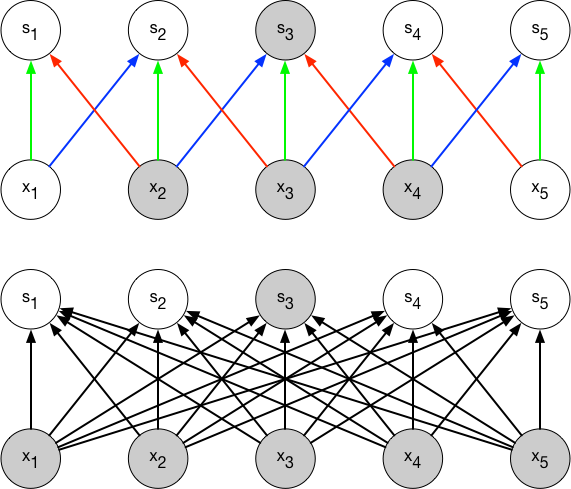
\includegraphics[width=0.6\textwidth]{assets/conv_1d.png}
	\caption{(\textit{Oben})1D Convolution mit \textit{kernel} der Grösse 3. $s_3$ wird durch 3 inputs beeinflusst.
		     (\textit{Unten}) \textit{Dense Network}. $s_3$ wird durch alle inputs beeinflusst.\parencite{goodfellow}}
	\label{img:conv}
\end{figure}

Ein weiterer Vorteil von \textit{Convolutional Neural Networks} ist, dass sie eine räumliche Hyrarchie von Mustern erlernen können. Wenn die Eingabe das Bild einer Katze ist, wird zum Beispiel die erste Schicht unterschiedliche Kanten erkennen, die zweite Schicht dann einzelne Merkmale (z.b Augen), und so weiter.

Damit das gilt, muss aber der analysierte Bereich eines Knotens, von Schicht zu Schicht grösser werden. Deshalb wird meisten nach jedem \textit{Convolution Layer} ein \textit{Pooling Layer} gesetzt. Das \textit{Pooling Layer} fasst mehrere Datenpunkte zusammen um dem nächsten Netzwerk eine grösseren Analysebereich zu verschaffen. Ein oft verwendetes Pooling-Verfahren ist \textit{Max-Pooling}: Angrenzende Knoten werden zusammengefasst durch ihr Maximum. \index{Max-Pooling}
\begin{figure}[hbt]
	\centering
		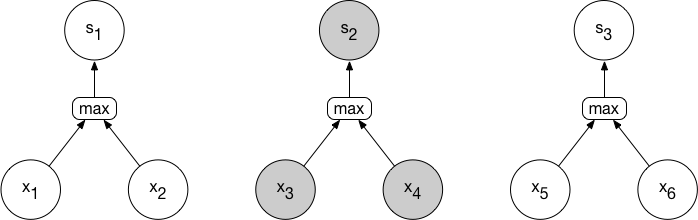
\includegraphics[width=0.75\textwidth]{assets/pooling_1d.png}
	\caption{1D Max-Pooling layer: z.B $s_2$ ist $\max (x3, x4)$}
	\label{img:pool}
\end{figure}


\subsection{Recurrent Neural Networks}
Eine gemeinsame Eigenschaft von allen \textit{Dense Neural Networks} und CNN's ist, dass sie keinen Speicher haben. Bei jedem Vorwärtspass berechnet das Netzwerk alles von neuem ohne Erinnerungen an vorherige Durchlaufe. Dieses Verhalten ist das absolute Gegenteil vom menschlichem Denkprozess. Wenn wir einen Satz lesen, durchgehen wir ihn Wort nach Wort und merken uns den vorherigen Kontext.

\textit{Recurrent Neural Networks} (RNN) bilden diesen Prozess vereinfacht nach. Sie besitzen eine interne wiederkehrende Schleife die dem Netzwerk Informationen aus dem vorherigen Durchlauf bereitstellt (Siehe Abbildung \ref{img:rnn_loop}). Die RNN Zelle berechnet dann die nächste Ausgabe sowohl aus der neuen Eingabe, wie auch mit den Erinnerungen der letzten Ausgabe. \parencite{chollet}\\
\begin{figure}[hbt]
	\centering
		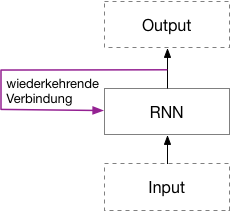
\includegraphics[width=0.35\textwidth]{assets/rnn_loop.png}
	\caption{RNN mit Schlaufe}
	\label{img:rnn_loop}
\end{figure}

Der Vorgang lässt sich grafisch über die Zeit aufgerollt darstellen (Abbildung \ref{img:rnn_unrolled}). In dieser Darstellung fällt auf, dass das Netzwerk theoretisch für jeden Schritt eine Ausgabe besitzt. Die zwischenliegenden Ausgaben sind vor allem wichtig, wenn man eine weitere Schicht an das Netzwerk anhängen will. Sonst behält man meist nur die letze Ausgabe, da diese indirekt Informationen über alle anderen beinhaltet.\\
\begin{figure}[hbt]
	\centering
		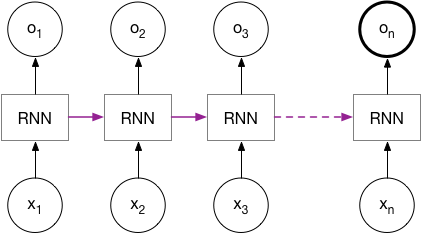
\includegraphics[width=0.67\textwidth]{assets/rnn_unrolled.png}
	\caption{RNN aufgerollt über die Zeit}
	\label{img:rnn_unrolled}
\end{figure}

Das ganze Prinzip ergibt jedoch nur Sinn, wenn frühere Eingaben tatsächlich einen Einfluss auf spätere Ausgaben haben. Eine praktische Anwendung ist das Verarbeiten von zeitlichen Sequenzen wie Wetterdaten und Sprache. Die einzelnen Lernbeispiele werden  zeitlich zerteilt und stückweise dem Netzwerk gefüttert.
Eine fortgeschrittene Implementation von RNN Zellen ist unter anderem die \textit{Long short-tem memory} (LSTM) Zelle \parencite{schmidhuber}. Durch das Einführen von unterschiedlichen wiederkehrenden Verbindungen wird verhindert, dass ältere Signale langsam verschwinden, bzw. vergessen werden \parencite{chollet}.
	\section{Daten}


\subsection{Datenquellen}
Es gibt keine frei zugänglichen umfassenden Datensets für Sprachidentifikation. Datensets wie das \textit{NIST Language Recognition Evaluation}\cite{nist} sind nur unter teuren Gebühren zugänglich. Wie verwandte Arbeiten empfehlen \cite{iLID}, wird darum ein eigenes Datenset zusammengestellt. Es werden gleichmässig Daten zu den Sprachen Deutsch, Englisch, und Französisch gesammelt. Die Daten stammen vom \textit{Voxforge}\cite{voxforge} Datenset, von \textit{Youtube}\cite{youtube} und von \textit{Librivox}\cite{librivox}.

\paragraph{Voxforge} ist ein open-source Datenset für Spracherkennung. Es besteht aus vielen kurzen (1-10s), von Benutzern hochgeladenen, Audiodateien. Die englische Sprache dominiert mit rund 120h Audio das Datenset. Über alle drei Sprachen verteilt sind 190 Stunden Ton verfügbar. Die Audioqualität variiert je nach Benutzer.

Die Sprache ist langsam und deutlich verständlich. Sie hört sich eher künstlich an im Vergleich zu einem natürlichem Gespräch. Die Anzahl unterschiedlicher Sprecher ist gering.

\paragraph{Youtube}dient als Quelle für abwechslungsreiche Sprache. Es werden populären Nachrichtenkanäle wie CNN, ARD, etc. verwendet (Siehe Tabelle \ref{tab:channels}). Die Aufnahmen werden oft von diversen Hintergrundgeräuschen begleitet und die Variation der Sprecher gross, da oft fremde Gäste eingeladen werden. Kehrseite ist, dass nicht garantiert werden kann, dass alle Aufnahmen tatsächlich die richtige Sprache beinhalten. Sendepausen und fremdsprachige Interviews kommen vereinzelt vor.
\begin{table}[h]
        \centering
        \begin{tabular}[t]{l || l}
        Sprache & Kanäle \\
        \hline \hline
        Französisch & France24, FranceInfo\\
        Deutsch & ARD, ZDF\\
        Englisch & CNN,  BBC
        \end{tabular}
        \caption{Youtube Kanäle}
        \label{tab:channels}
\end{table}

\paragraph{Librivox} ist ein öffentlich abrufbares Hörbuch Datenset. Anstatt selbst Hörbücher zu selektieren, wird eine vorgefertigte Selektion verwendet \cite{librivox-compilation}. Verfügbar sind sieben Stunden Aufnahmen mit 90 verschiedenen Sprechern.


\subsection{Daten Auswahl}
Die Modelle werden grundsätzlich mit den Daten von Voxforge und Youtube trainiert und ausgewertet. Es werden zwei unterschiedliche Datenquellen verwendet um die \textit{Stichprobenverzerrung} zu minimieren. Stichprobenverzerrung bedeutet, dass das Datenset nicht repräsentativ für alle Sprachaufnahmen ist. Bei Voxforge ist zum Beispiel die Gefahr, dass das Modell sich überanpasst an die geringe Anzahl Sprecher. Anstatt die Sprache zu erkennen, könnte das Modell das Mikrofon des Sprechers identifizieren und jedem Sprecher eine Sprache zuordnen. Die Leistung des Modells für neue Sprecher wäre dann nicht besser als ein Zufallsgenerator.
\\
Um die Stichprobenverzerrung zu messen werden die Modelle zusätzlich auf dem Librivox Datenset ausgewertet. Die Daten von Librivox teilen keine systematischen "Fehler" wie zum Beispiel Sprecher mit den Trainingsdaten. Das Librivox-Testset besteht aus insgesamt 2 Stunden Aufnahmen.
\\
Von Youtube und Voxforge werden gemeinsam 139 Stunden Audiodaten heruntergeladen, was 100'000 5s Aufnahmen entspricht. Die Datenmenge wird bewusst klein gehalten, weil grössere Datenmengen ressourcenaufwändiger und ineffizienter wären. Die einzelnen Sprachen und Quellen sind zu gleichen Teilen repräsentiert. 
\\
Die Daten werden weiter in 80\% Trainingsdaten, 10\% Testdaten und 10\% \textit{Validationset} gespalten. Das Validationset wird verwendet um während dem Training zu beobachten, wie das Modell auf neue Daten reagiert. Die \textit{Hyperparamter} \index{Hyperparameter}(Parameter die das Netzwerk nicht selber lernen kann, z.B die Anzahl Knoten) werden manuell so angepasst dass das Netzwerk möglichst gut auf dem Validationset abschneidet. Tabelle \ref{tab:data} gibt eine Übersicht über die Verteilung der Daten.
\begin{table}[]
	\centering
	\begin{tabular}{llll}
	\hline
	Netz          & Voxforge & Youtube & Librivox \\ \hline
	Trainingset   & 56h      & 56h     & -        \\
	Validationset & 7h       & 7h      & -        \\
	Testset       & 7h       & 7h      & 2h       \\ \hline
	\end{tabular}
	\caption{Daten Verteilung}
	\label{tab:data}
\end{table}


\subsection{Preprocessing}
Sprache besteht aus Wörtern und Wörter sind grundsätzlich eine Abfolge von Lauten. Verschiedene Sprachen unterscheiden sich an den verschiedenen Abfolgen von Lauten, manchmal sogar an den verwendeten Lauten selbst. Die kleinste relevante Einheit für Spracherkennung, sowohl für den Menschen wie die Maschine, ist also ein Laut.

Wenn der Computer mit dem Mikrofon aufnimmt, misst er kleinste Druckunterschiede, bzw. Schallwellen. Eine unkomprimierte Audiodatei zeigt den Schalldruck über die Länge der Aufnahme, siehe Abbildung \ref{img:preprocessing} \textit{(oben)}.
Die einzelne Schallwelle ist für den Menschen nicht erkennbar, deshalb ist sie auch für die Sprache von keiner Bedeutung. Erst mehrere Schallwellen, bzw. die daraus folgende Frequenz lässt sich als Laut hören. 

Das Verfahren um aus einer Schallwelle die unterschiedlichen Frequenzen zu bestimmen heisst \textit{Fourier-Transformation} \cite{fourrier}. Falls dem Netzwerk als Eingabe rohe Schallwellen gefüttert werden, muss es dieses Verfahren erlernen, um dann aus den Lauten die Sprache erkennen zu können. Allerdings ist die Fourrier-Transformation zu erlernen ein zusätzlicher Aufwand und fordert den Computer darum mehr. Um dem Algorithmus die Aufgabe zu erleichtern, kann man ihm darum als Eingabe die berechneten Laute anstatt der rohen Schallwelle geben.

Die Prozedur dem Algorithmus bereits vorgerechnete Werte zu füttern, heisst \textit{Preprocessing} \index{Preprocessing}und ist weit verbreitet im Feld von \textit{Machine learning}. Das Vorrechnen ist unter dem Namen \index{Feature Engineering}\textit{Feature Engineering} bekannt. \textit{Features}, also Merkmale z.b Laute werden aus den Rohen Daten extrahiert. \parencite[vgl.][]{chollet}

\subsubsection{Spektrogramme}
\begin{figure}[hbt]
	\centering
		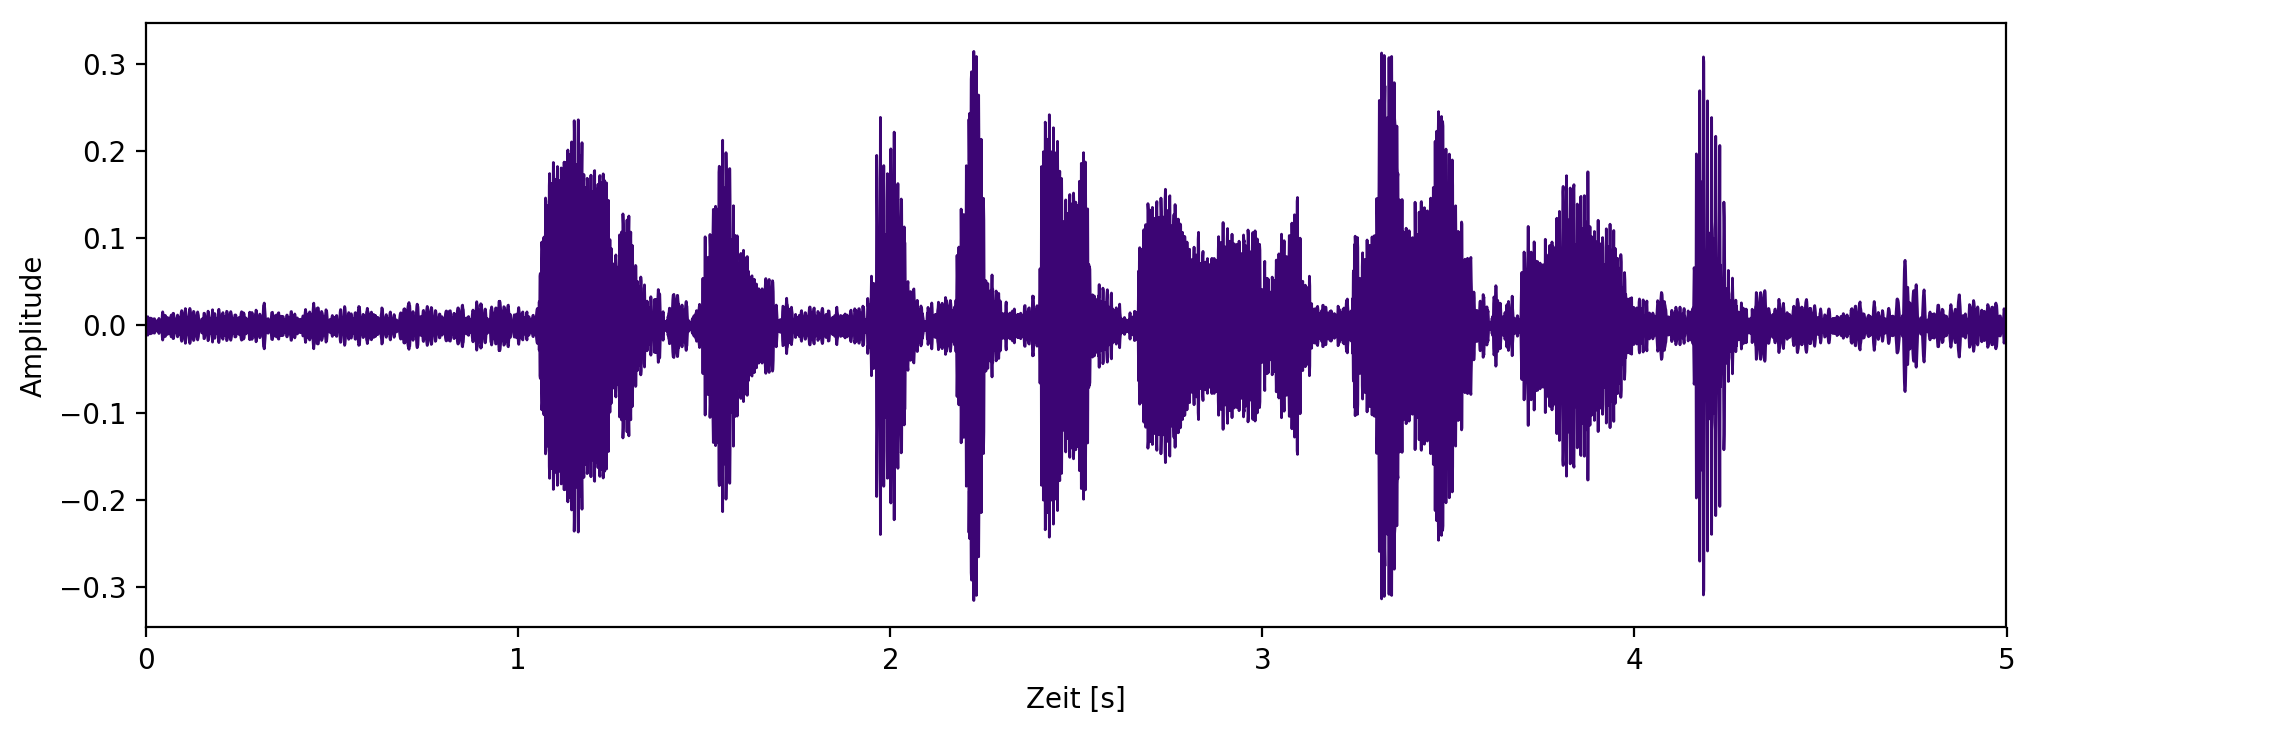
\includegraphics[width=0.6\textwidth]{assets/audio_raw.png}
		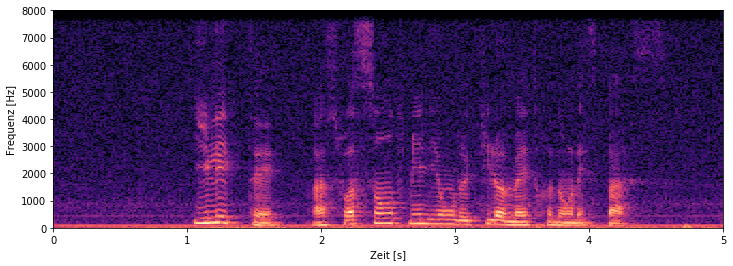
\includegraphics[width=0.6\textwidth]{assets/audio_log.png}
		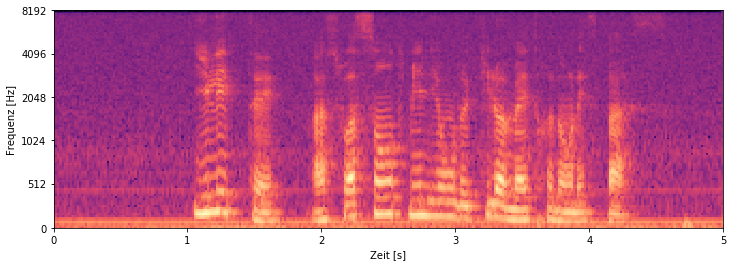
\includegraphics[width=0.6\textwidth]{assets/audio_mel.png}
	\centering
	\caption{Audio-Preprocessing: \textit{(oben)} Rohe Schallwelle, \textit{(mitte)}
		     Dezibel-Spectrogramm, 
		     \textit{(unten)} Mel Dezibel-Spectrogramm}
	\label{img:preprocessing}
\end{figure}
Spektrogramme \index{Spektrogramme}sind grafische Darstellungen eines Hörsignals nach der Anwendung der Fourrier-Transformation\parencite[]['Spectrograms']{fourrier}, ersichtlich in Abbildung \ref{img:preprocessing} \textit{(Mitte)}. Frequenzen über 10kHz können abgeschnitten werden, da menschliche Sprache grösst Teils darunter abläuft\parencite{tenkHz}. Im Spektrogramm lassen sich von Auge Muster erkennen und unterscheiden. Der visuelle Charakter der Spektrogramme erlaubt ausserdem das verwenden von \textit{Convolutional Neural Networks}.

\subsubsection{Mel Filtering}

Spektrogramme haben relativ viele Datenpunkte und sind deshalb recht aufwändig zu verarbeiten. Ein weiter \textit{preprocessing} Schritt wird deshalb oft angewendet: \textit{Mel Filtering}\parencite{mel}. Die Frequenzen werden dabei in grössere Eimer gepackt. Unter 1kHz sind die Eimer linear verteilt und darüber logarithmisch, siehe Abbildung \ref{img:preprocessing} \textit{(unten)}. Das Modell entspricht unserer Hörfähigkeit, die recht präzise unter 1kHz arbeitet, höhere Frequenzen aber schlecht unterscheiden kann\parencite{tenkHz}. 

\subsubsection{Implementation}

Die Oben genannten Transformationen können vor dem Training direkt auf die Daten angewendet und abgespeichert werden. In diesem Fall hätte man die rohen Daten löschen können. Allerdings sollte in dieser Arbeit sowohl an den rohen Daten wie auch an der Transformation flexibel experimentiert werden können, weswegen die Daten unbedingt beibehalten werden mussten. 

Anstatt die Transformationen selber zu implementieren wird ein Framework verwendet. In diesem Fall bietet sich an \textit{kapre}\parencite{kapre} an. Mit Kapre lassen sich währende dem Training die Daten in Echtzeit verarbeiten. Das Training dauert dabei aber 20\% länger. Konkret verhält sich \textit{kapre} wie eine Schicht vor dem eigentlichen Neuronalen Netzwerk.
\begin{figure}[hbt]
	\centering
		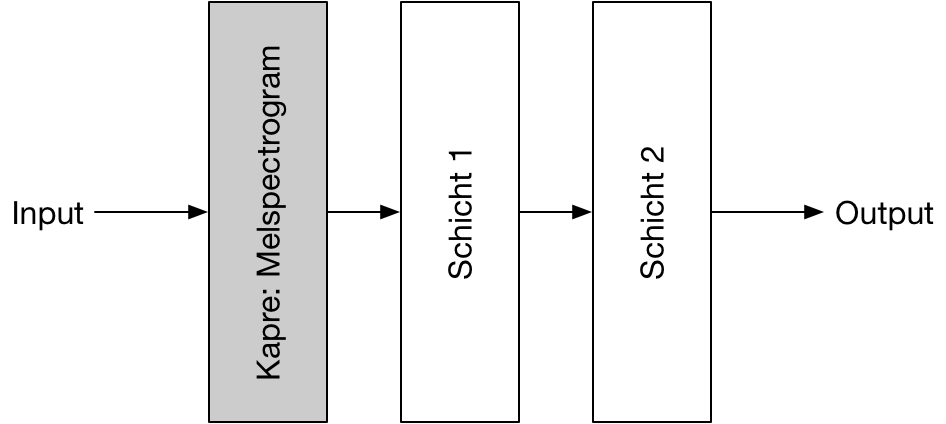
\includegraphics[width=0.6\textwidth]{assets/kapre.png}
	\centering
	\caption{\textit{Kapre}\parencite{kapre} als Schicht}
	\label{img:kapre}
\end{figure}


	\section{Web Interface}
Es war seit Anfang an klar, dass ein Web-Interface gestaltet werden sollte. Das Web-Interface ist ideal um die Leistung der Software hautnah zu erleben. Man kann mit jedem internetfähigen Gerät (mit Mikrofon) darauf zugreifen.

Die Idee ist einfach. Man nimmt direkt im Browser eine kurze Audioaufnahme auf, lädt diese hoch zum Server, und dieser antwortet mit der geschätzten Sprache. Bevor man die Aufnahme hochlädt kann man sie optional selbst abspielen.
%\\ Aktuell läuft ein Web-Server unter: \url{jo.guru.ksz.ch/deeplid}


\subsection{Frontend}
\begin{figure}[hbt]
	\centering
		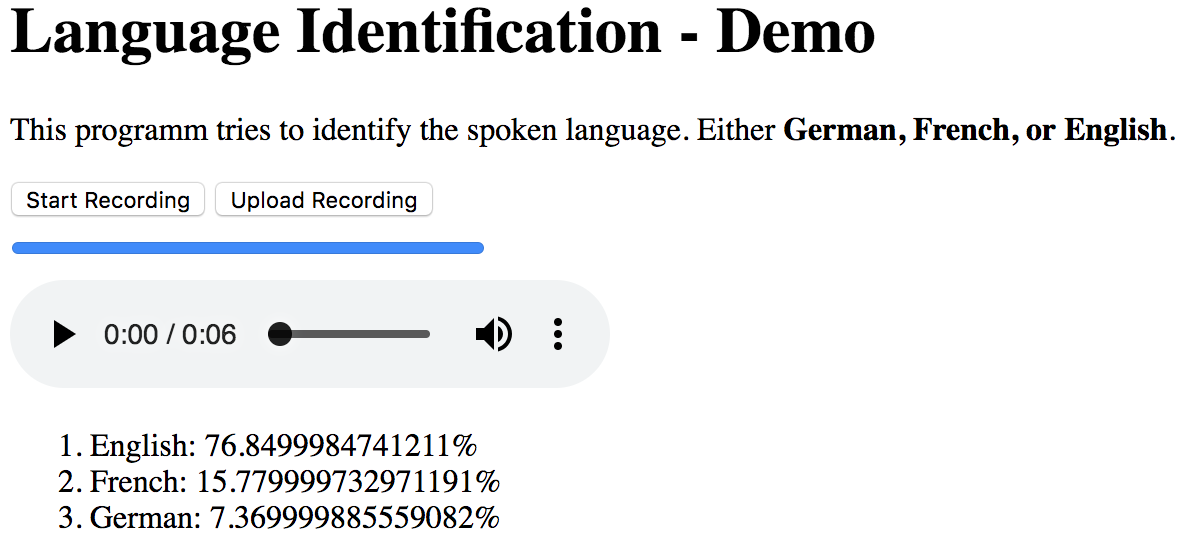
\includegraphics[width=0.6\textwidth]{assets/interface.png}
	\caption{Web-Interface Screenshot}
	\label{img:interface}
\end{figure}
Das Design ist in einfachem \textit{HTML} und \textit{CSS} geschrieben, die Logik mit \textit{Javascript}. Um im Browser Audioaufnahmen nehmen zu können, wird \textit{RecordRTC}\cite{recordrtc} verwendet. \textit{RecordRTC} ist eine unter der \textit{MIT} Lizenz veröffentlichte \textit{Javascript} Bibliothek für Medienaufnahmen. Sie ist kompatibel mit vielen modernen Browsern und Geräten.

Nach der Aufnahme wird die Datei über AJAX POST an den Server verschickt. Der Server antwortet mit einem XML-Snippet der Resultate.
Dieses wird wiederum direkt in die Webseite eingebaut.


\subsection{Backend}
Der Webserver läuft in der Programmiersprache \textit{Python}. Als Framework wird mit \textit{Flask}\cite{flask} verwendet. Da sowohl der \textit{Flask} wie auch \textit{Keras} mit Python laufen, kann der Webserver das trainierte Modell ohne zusätzliche Hürden verwenden.
Der Code findet sich unter \ref{code:webserver}

	\section{Resultate}
	\section{Diskussion}
	\subsection{Ausbaumöglichkeiten}
	\section{Code}


\subsection{Webserver}
\label{code:webserver}
\lstinputlisting[language=Python,
		      basicstyle=\small,
		      breaklines=true]{assets/code/server_snippet.py}

\subsection{Beispiel-Modell}
\lstinputlisting[language=Python,
		      basicstyle=\small,
		      breaklines=true]{assets/code/model_snippet.py}
	
	\printbibliography
	\listoffigures
\end{document}